\section{Simulação e choques}
\label{SecChoques}

Compreendidas as relações entre as variáveis através da solução analítica, resta simular o modelo. Nas subseções seguintes, são verificados os efeitos dos seguintes choques
(i) aumento na taxa de crescimento do investimento residencial ($\phi_0$ e $\dot p_h$); (ii) aumento na participação dos salários na renda e;  (iii) aumento na taxa de juro das hipotecas decorrente de um maior \textit{risk and trouble}. Antes de prosseguir, a figura \label{DAG} ilustra a hierarquia de determinação em que as setas vão das variáveis exógenas em direção às exógenas. A partir desta ilustração, fica visível a ausência de relação entre crescimento e distribuição bem como a forma com que os preços afetam o sistema por meio da taxa própria de juros e, consequentemente, a taxa de crescimento dos gastos autônomos. Dito isso, as simulações serão comparadas com um cenário \textit{baseline} representado pela linha tracejada e são resumidas na tabela \ref{Resumo_Simulacao}.

\begin{figure}[H]
	\centering
	\label{DAG}
	\caption{Diagrama representativo do modelo}
	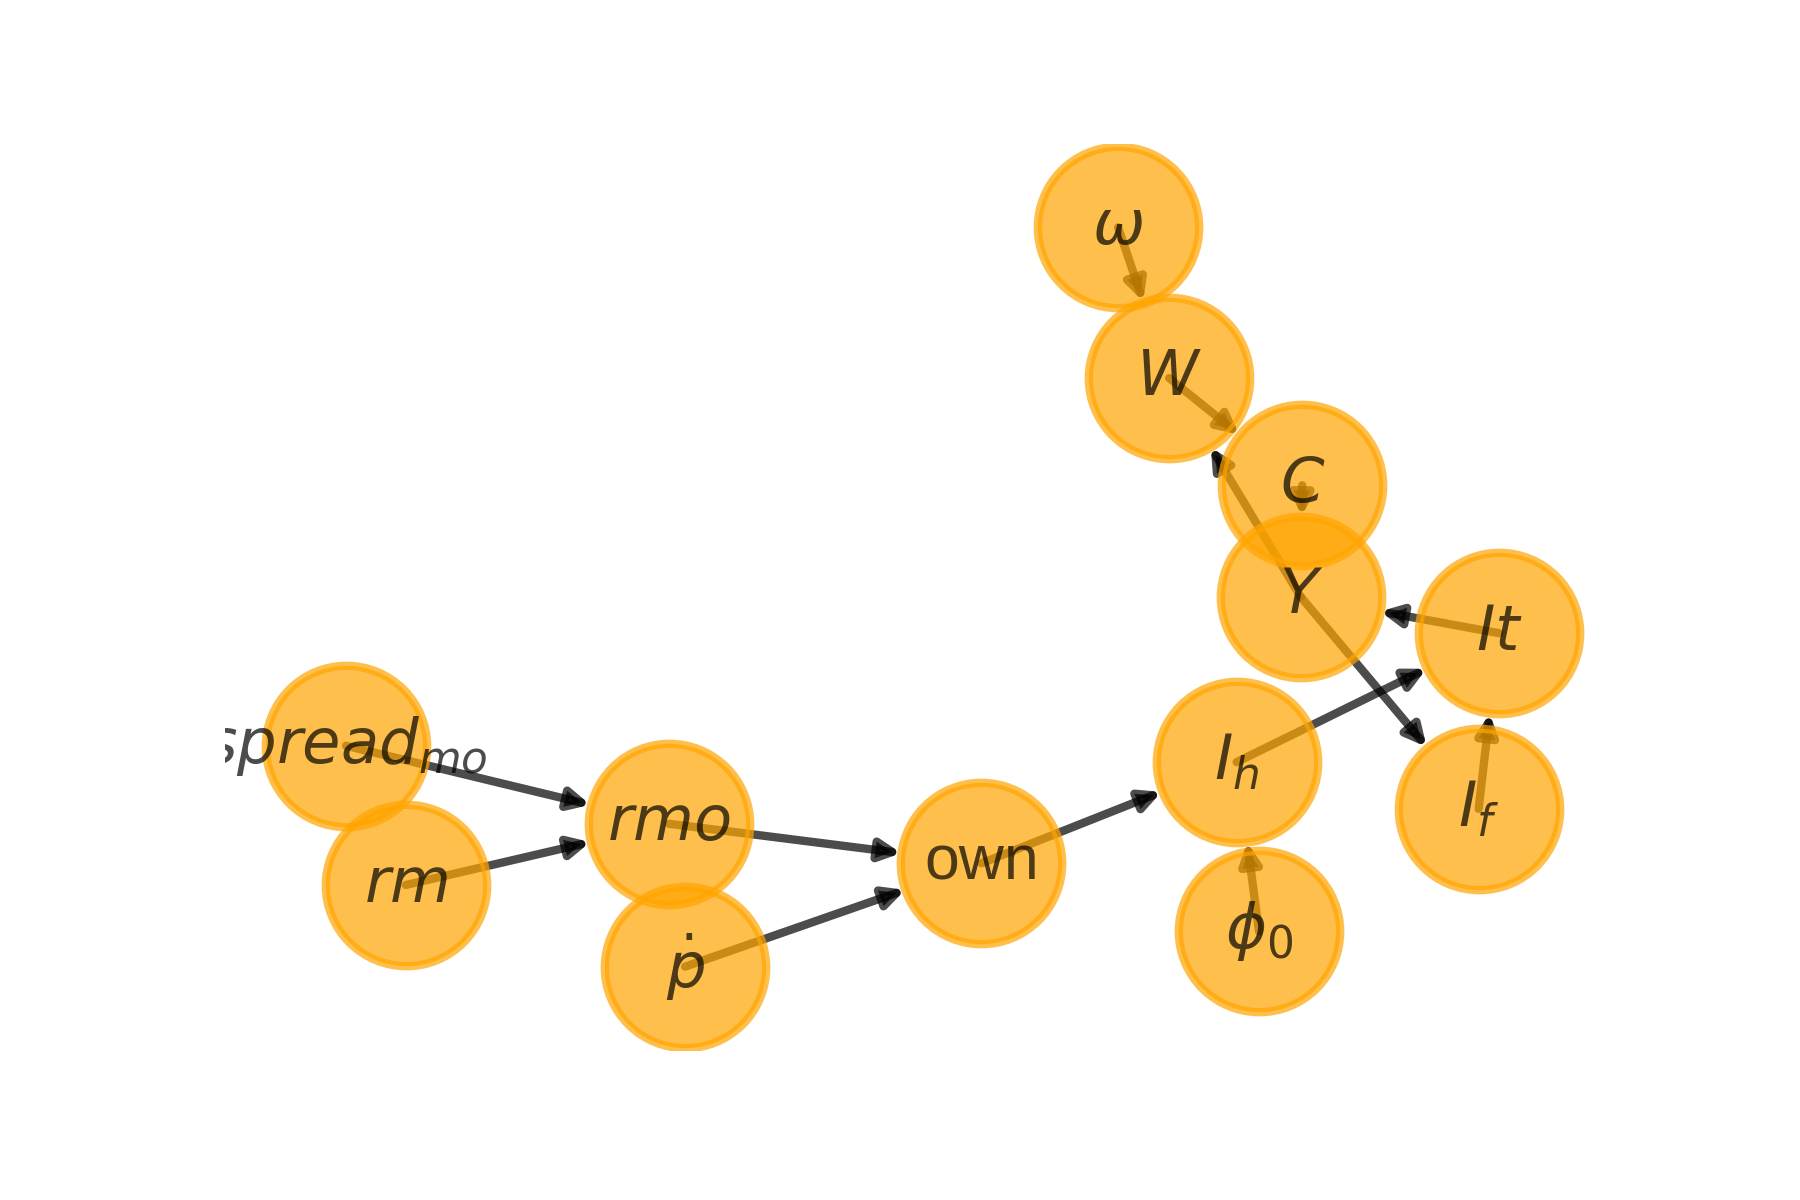
\includegraphics[width=\textwidth]{../../Modelo/Versoes/Dag.png}
	\caption*{\textbf{Fonte:} Elaboração própria}
\end{figure}



\subsection*{Aumento na taxa de crescimento do investimento residencial}

%Um aumento da taxa de crescimento dos gastos autônomos ($\uparrow g_Z$) causa uma maior taxa de crescimento da demanda que, por sua vez, implica em um maior grau de utilização. Em seguida, de acordo com o princípio do ajuste do estoque de capital, as firmas revisam seus planos de investimento e, consequentemente, altera a propensão marginal a investir de forma que o grau de utilização se ajusta lenta e gradualmente ao desejado. No longo prazo, (i) taxa de crescimento da economia converge a taxa dos gastos autônomos; (ii) como resultado, a propensão marginal a investir é permanentemente mais elevada em relação ao \textit{baseline}; (iii) grau de utilização converge ao normal.

Um aumento da taxa de crescimento dos gastos autônomos (seja por um aumento em $\phi_0$ ou na inflação de imóveis) significa uma maior taxa de crescimento da demanda que inicialmente implica um maior grau de utilização da capacidade produtiva. Em seguida, de acordo com o princípio do ajuste do estoque de capital, as firmas revisam seus planos de investimento e, consequentemente, alteram a propensão marginal a investir de forma que o grau de utilização se ajuste lenta e gradualmente ao desejado. A mudança da propensão marginal a investir faz com que temporariamente a economia cresça mais rápido que os gastos autônomos. Ao fim dos processos de ajustamento: a (i) taxa de crescimento da economia converge a taxa dos gastos autônomos; (ii) a propensão marginal a investir é permanentemente mais elevada em relação ao \textit{baseline}; (iii) grau de utilização converge ao normal.



\begin{figure}[H]
	\centering
	\caption{Efeito de um aumento no componente autônomo}
	\label{choque_1}
	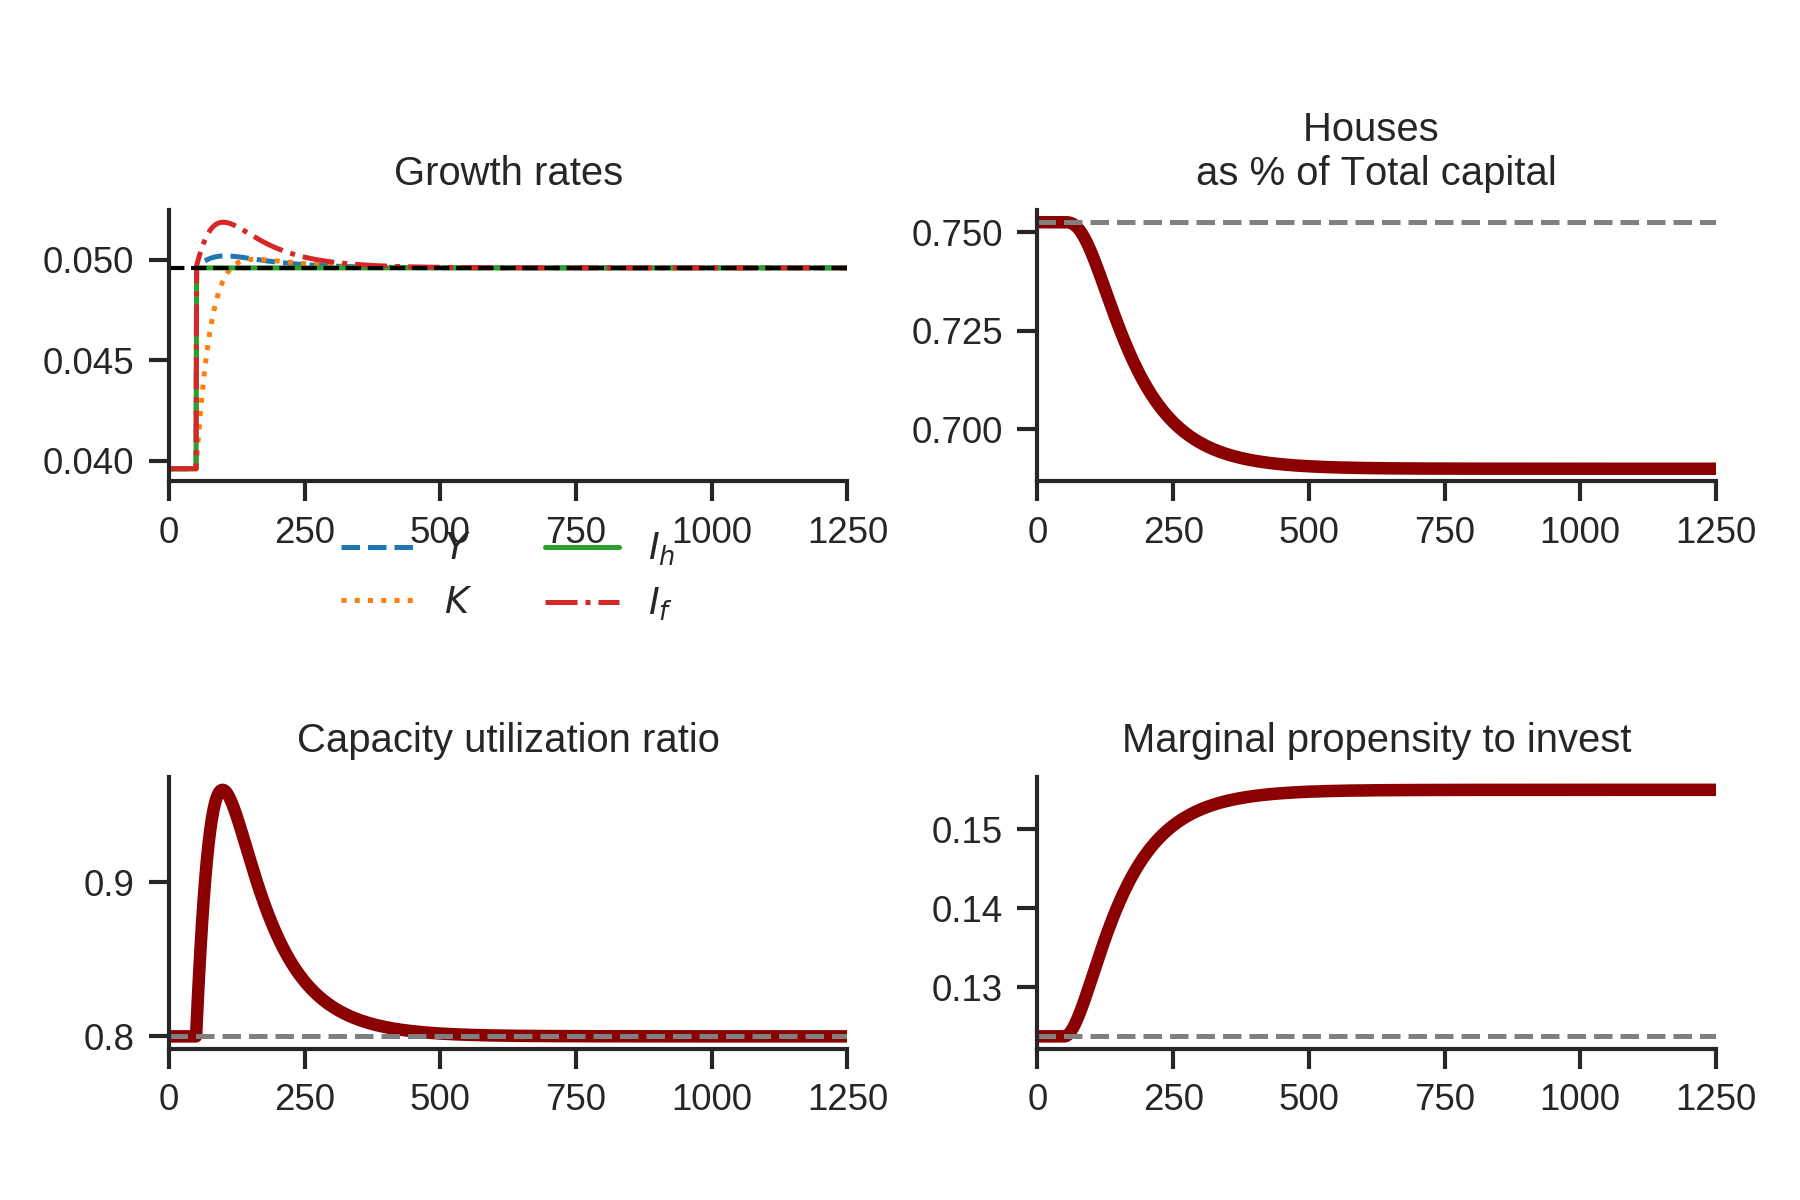
\includegraphics[width=\textwidth]{../../Modelo/Versoes/Shock_1.png}
	\caption*{\textbf{Fonte:} Elaboração própria}
\end{figure}


\begin{figure}[H]
	\centering
	\caption{Efeito de um aumento no componente autônomo}
	\label{choque_1Norms}
	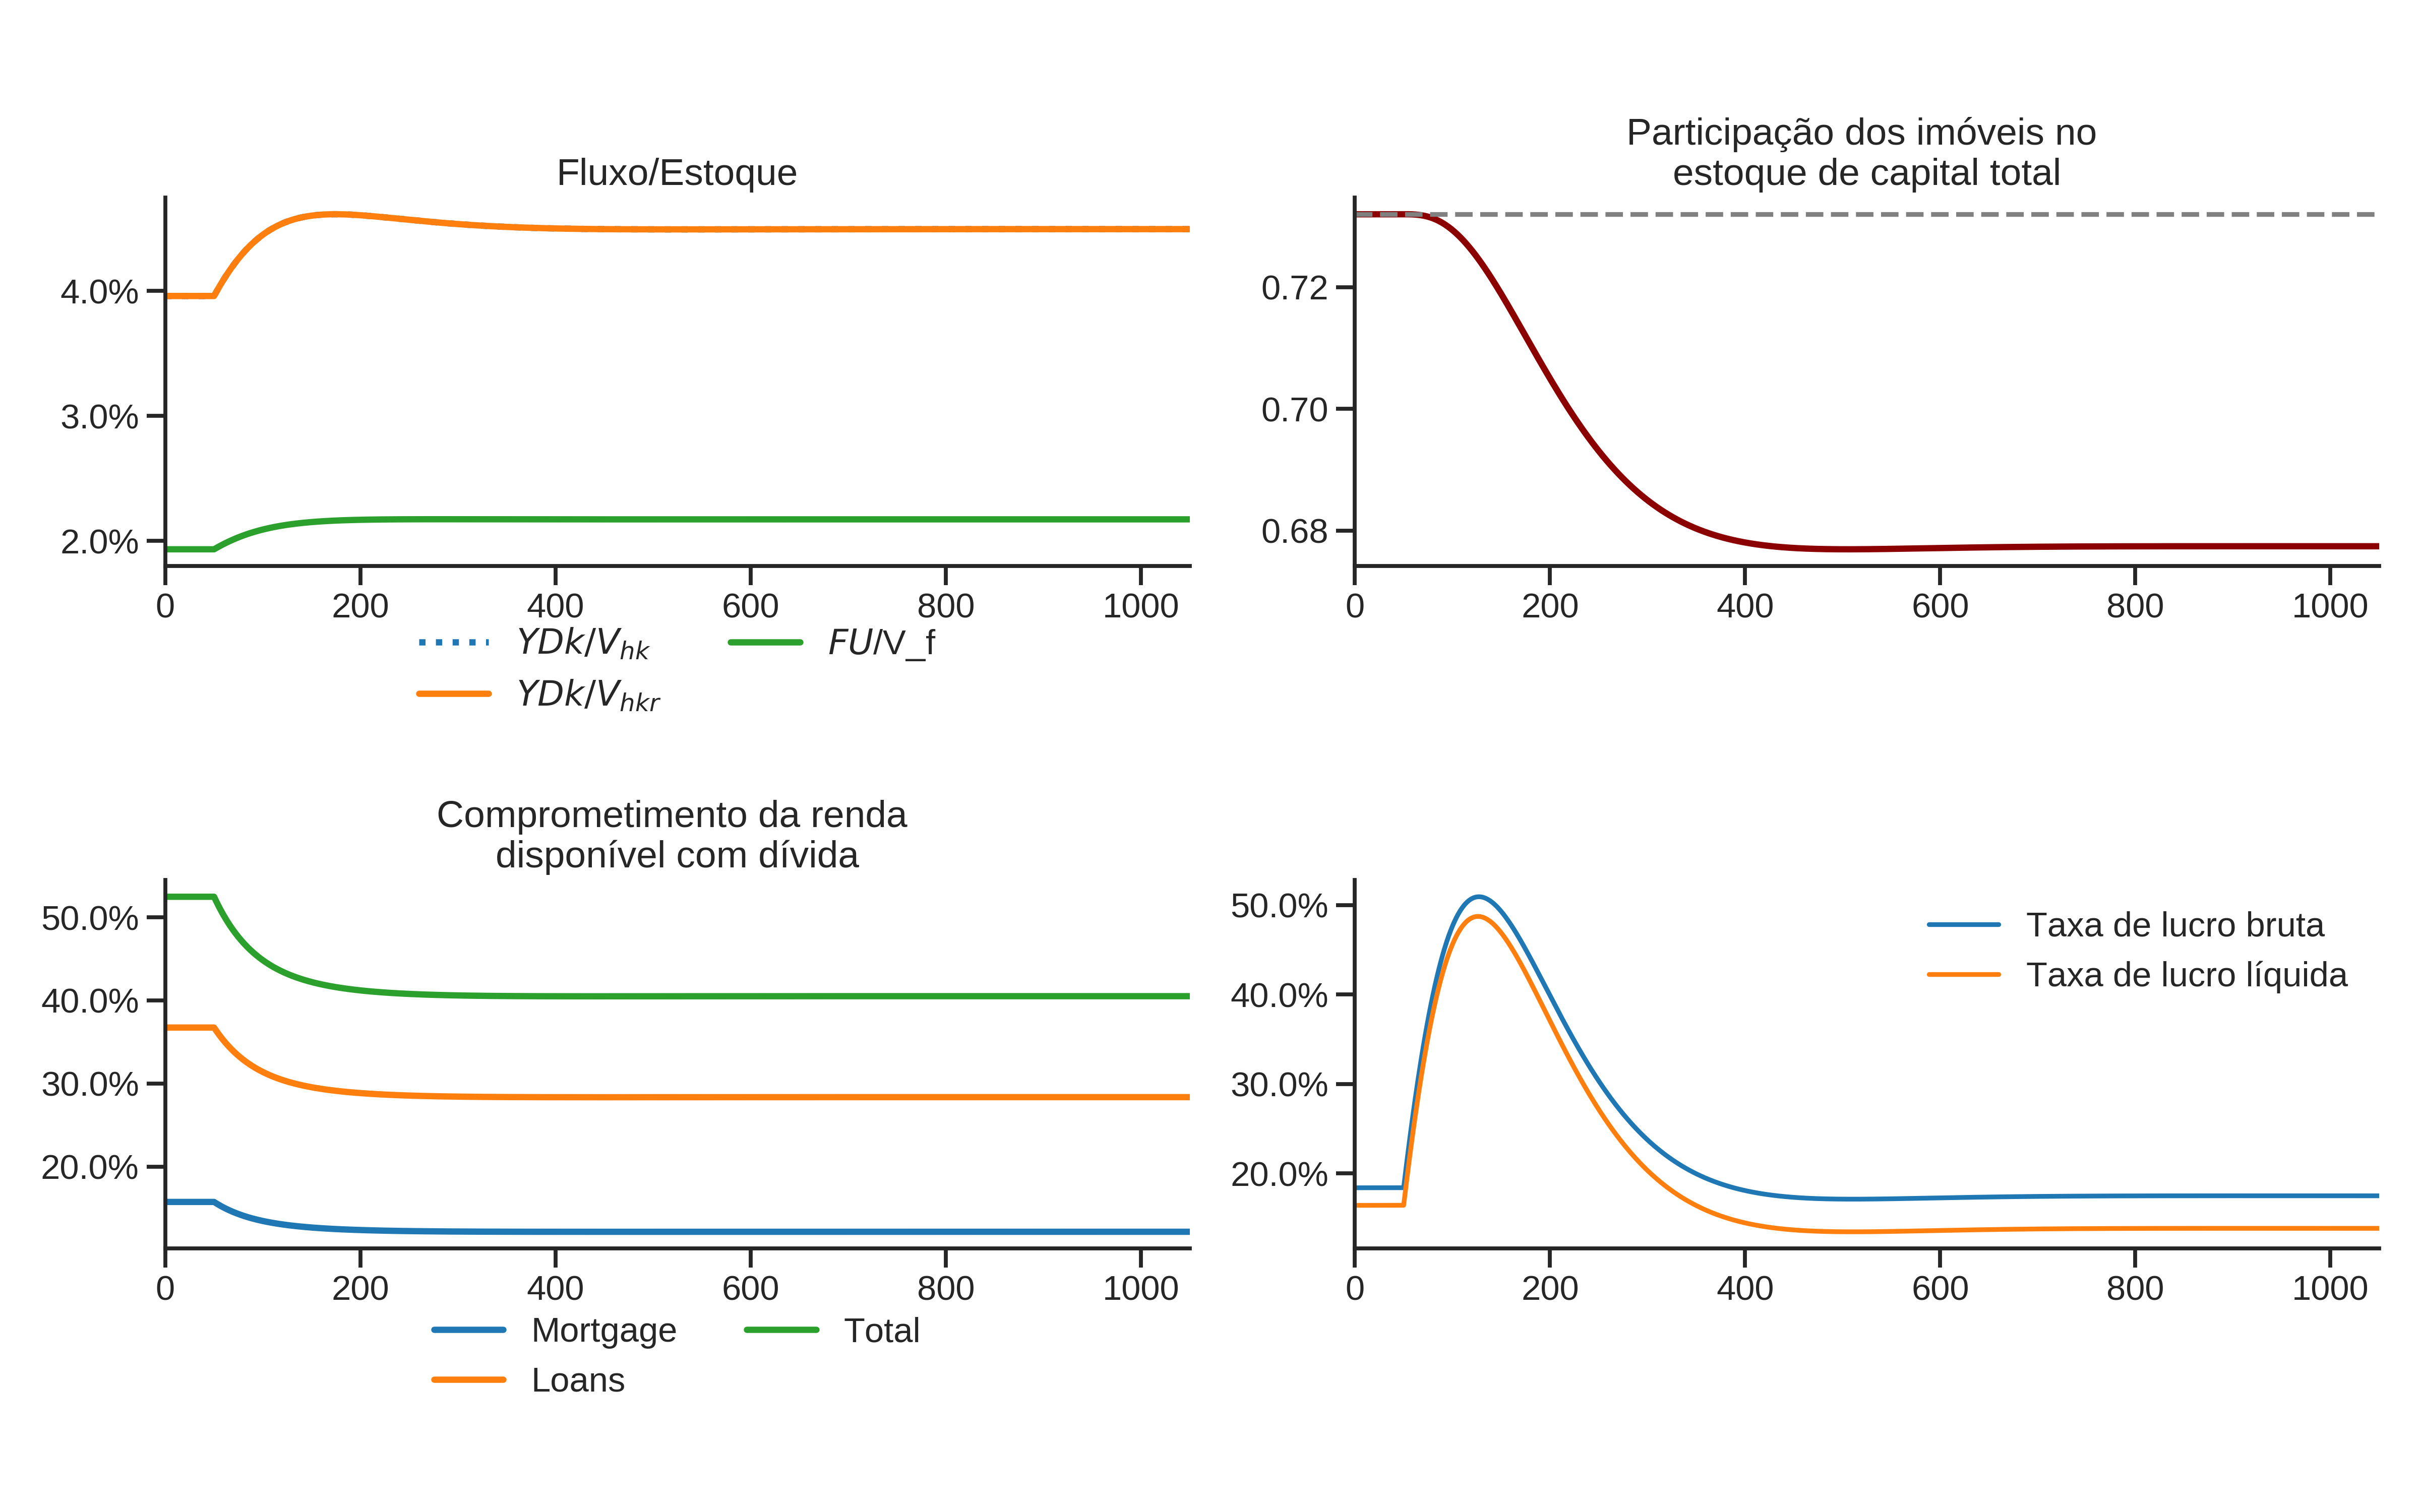
\includegraphics[width=\textwidth]{../../Modelo/Versoes/Shock_1Norms.png}
	\caption*{\textbf{Fonte:} Elaboração própria}
\end{figure}


\begin{figure}[H]
	\centering
	\caption{Efeito de um aumento da inflação de imóveis}
	\label{choque_4}
	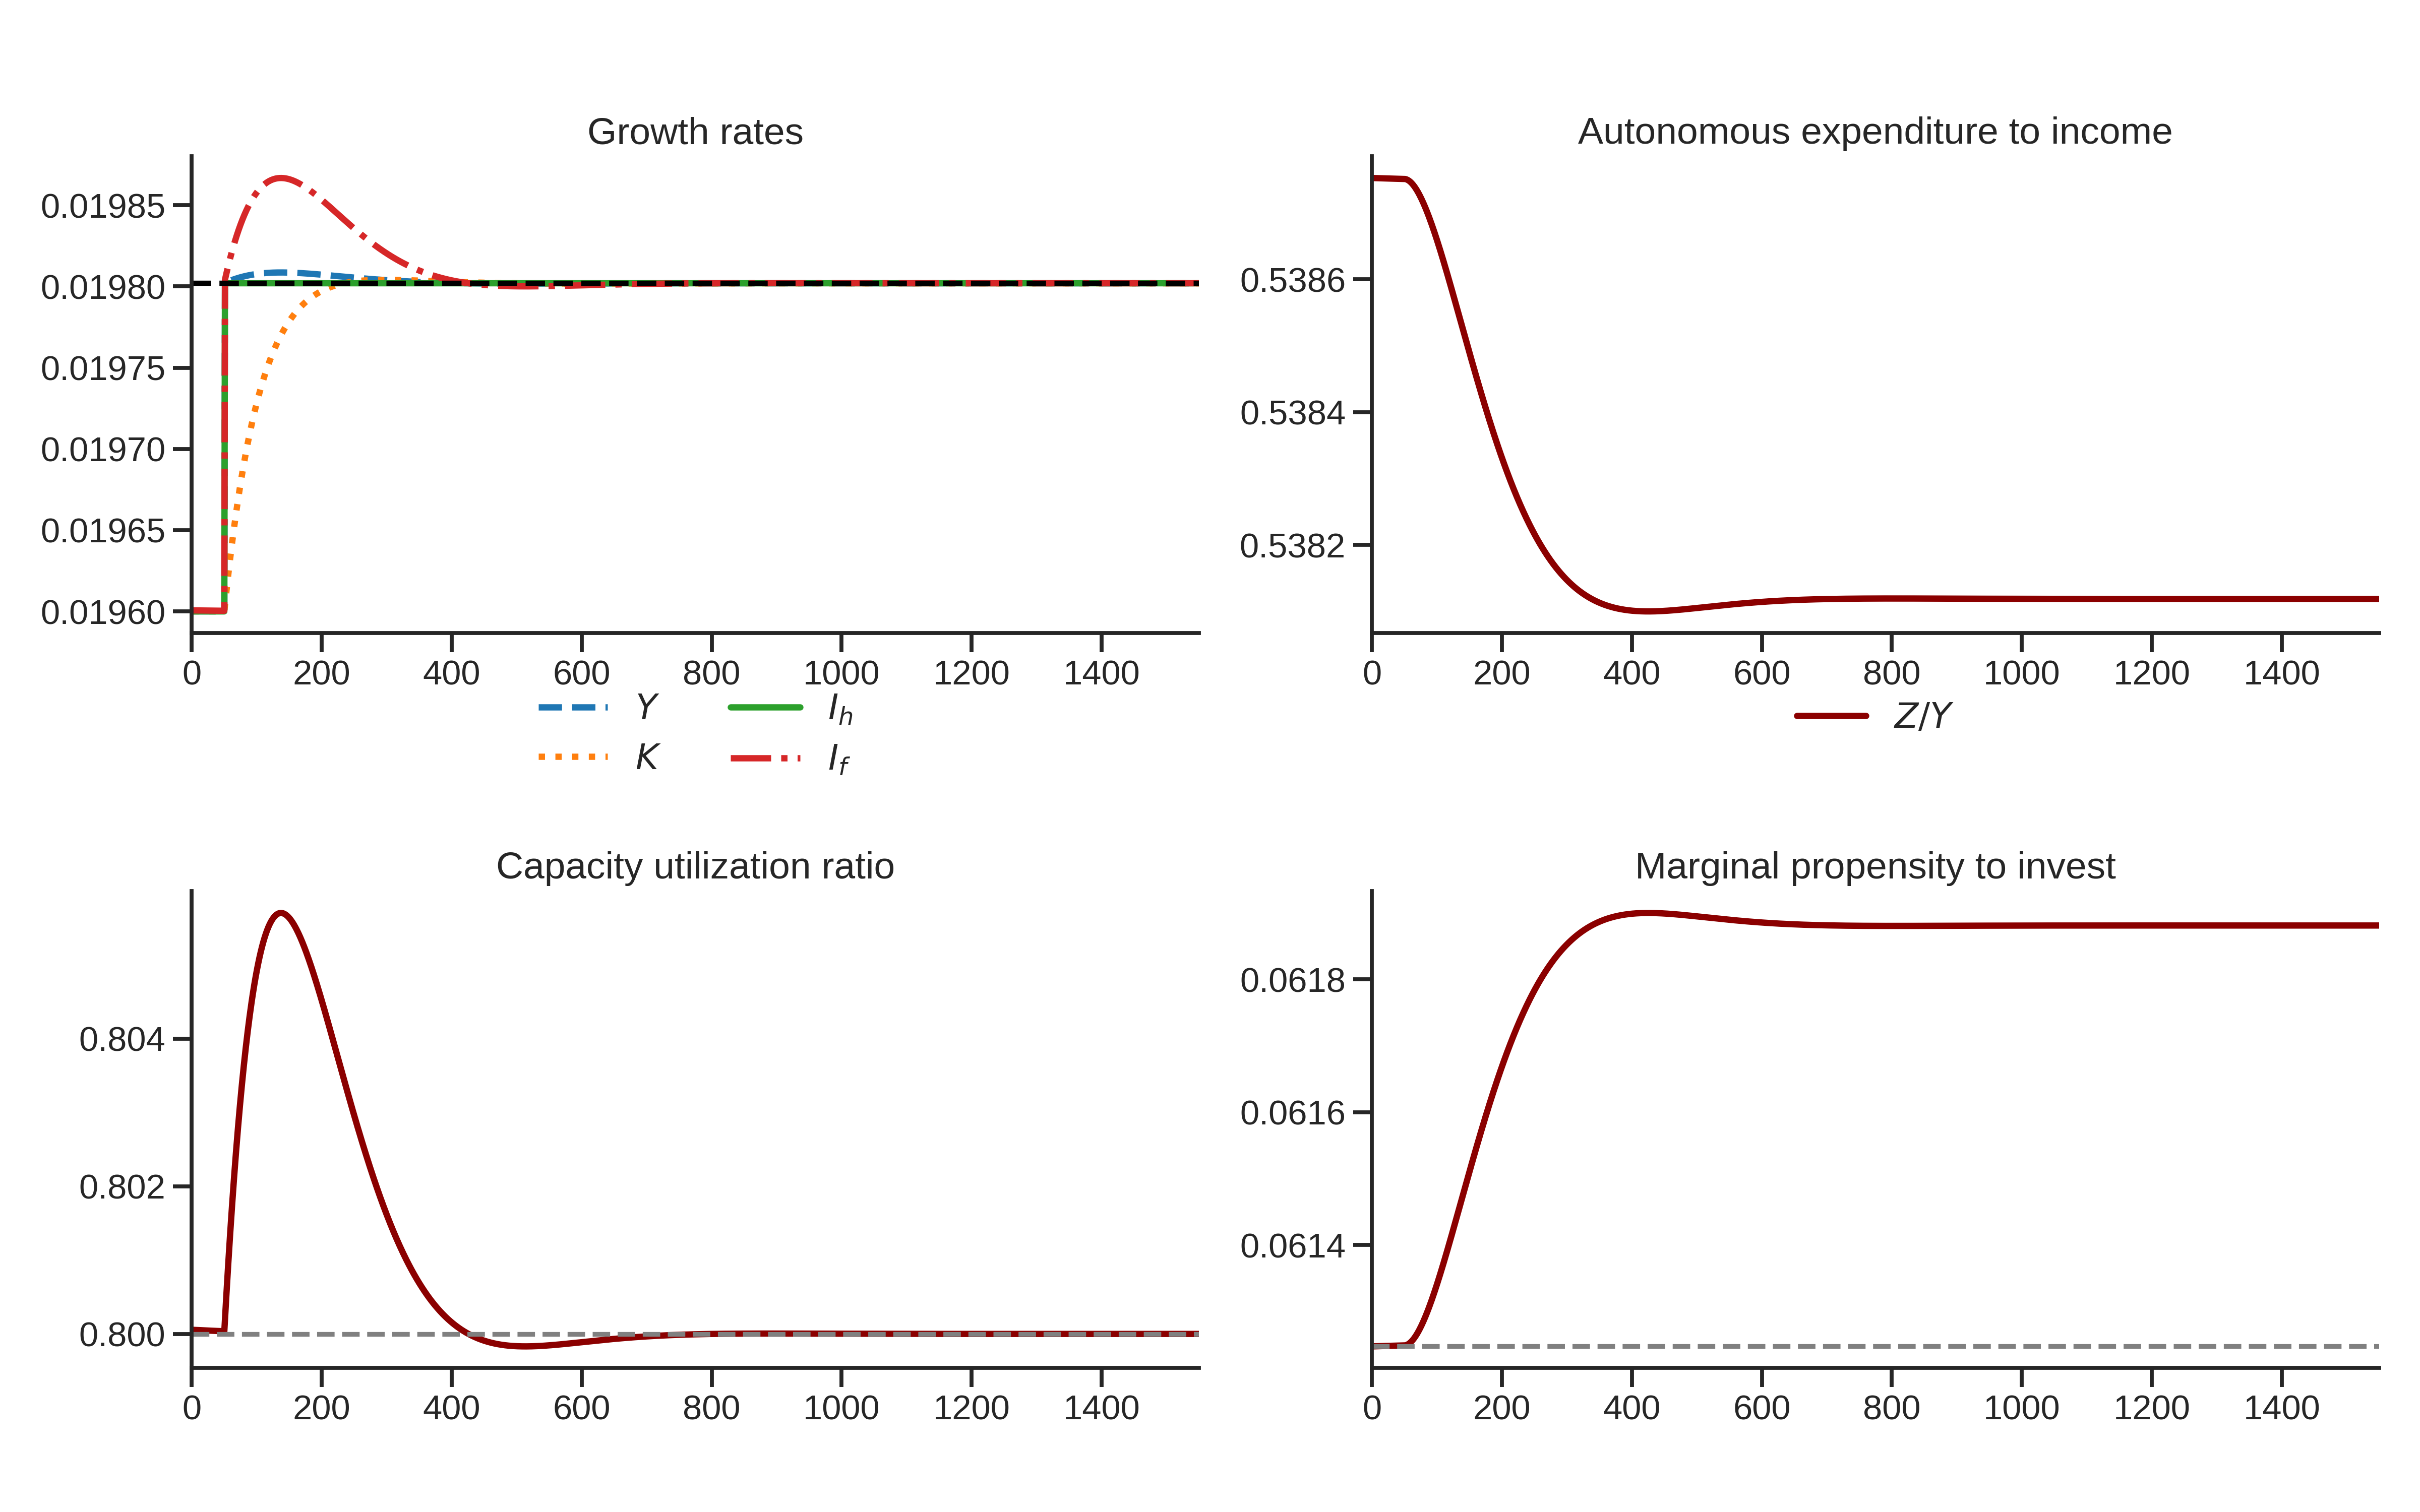
\includegraphics[width=\textwidth]{../../Modelo/Versoes/Shock_4.png}
	\caption*{\textbf{Fonte:} Elaboração própria}
\end{figure}


\begin{figure}[H]
	\centering
	\caption{Efeito de um aumento da inflação de imóveis}
	\label{choque_4Norms}
	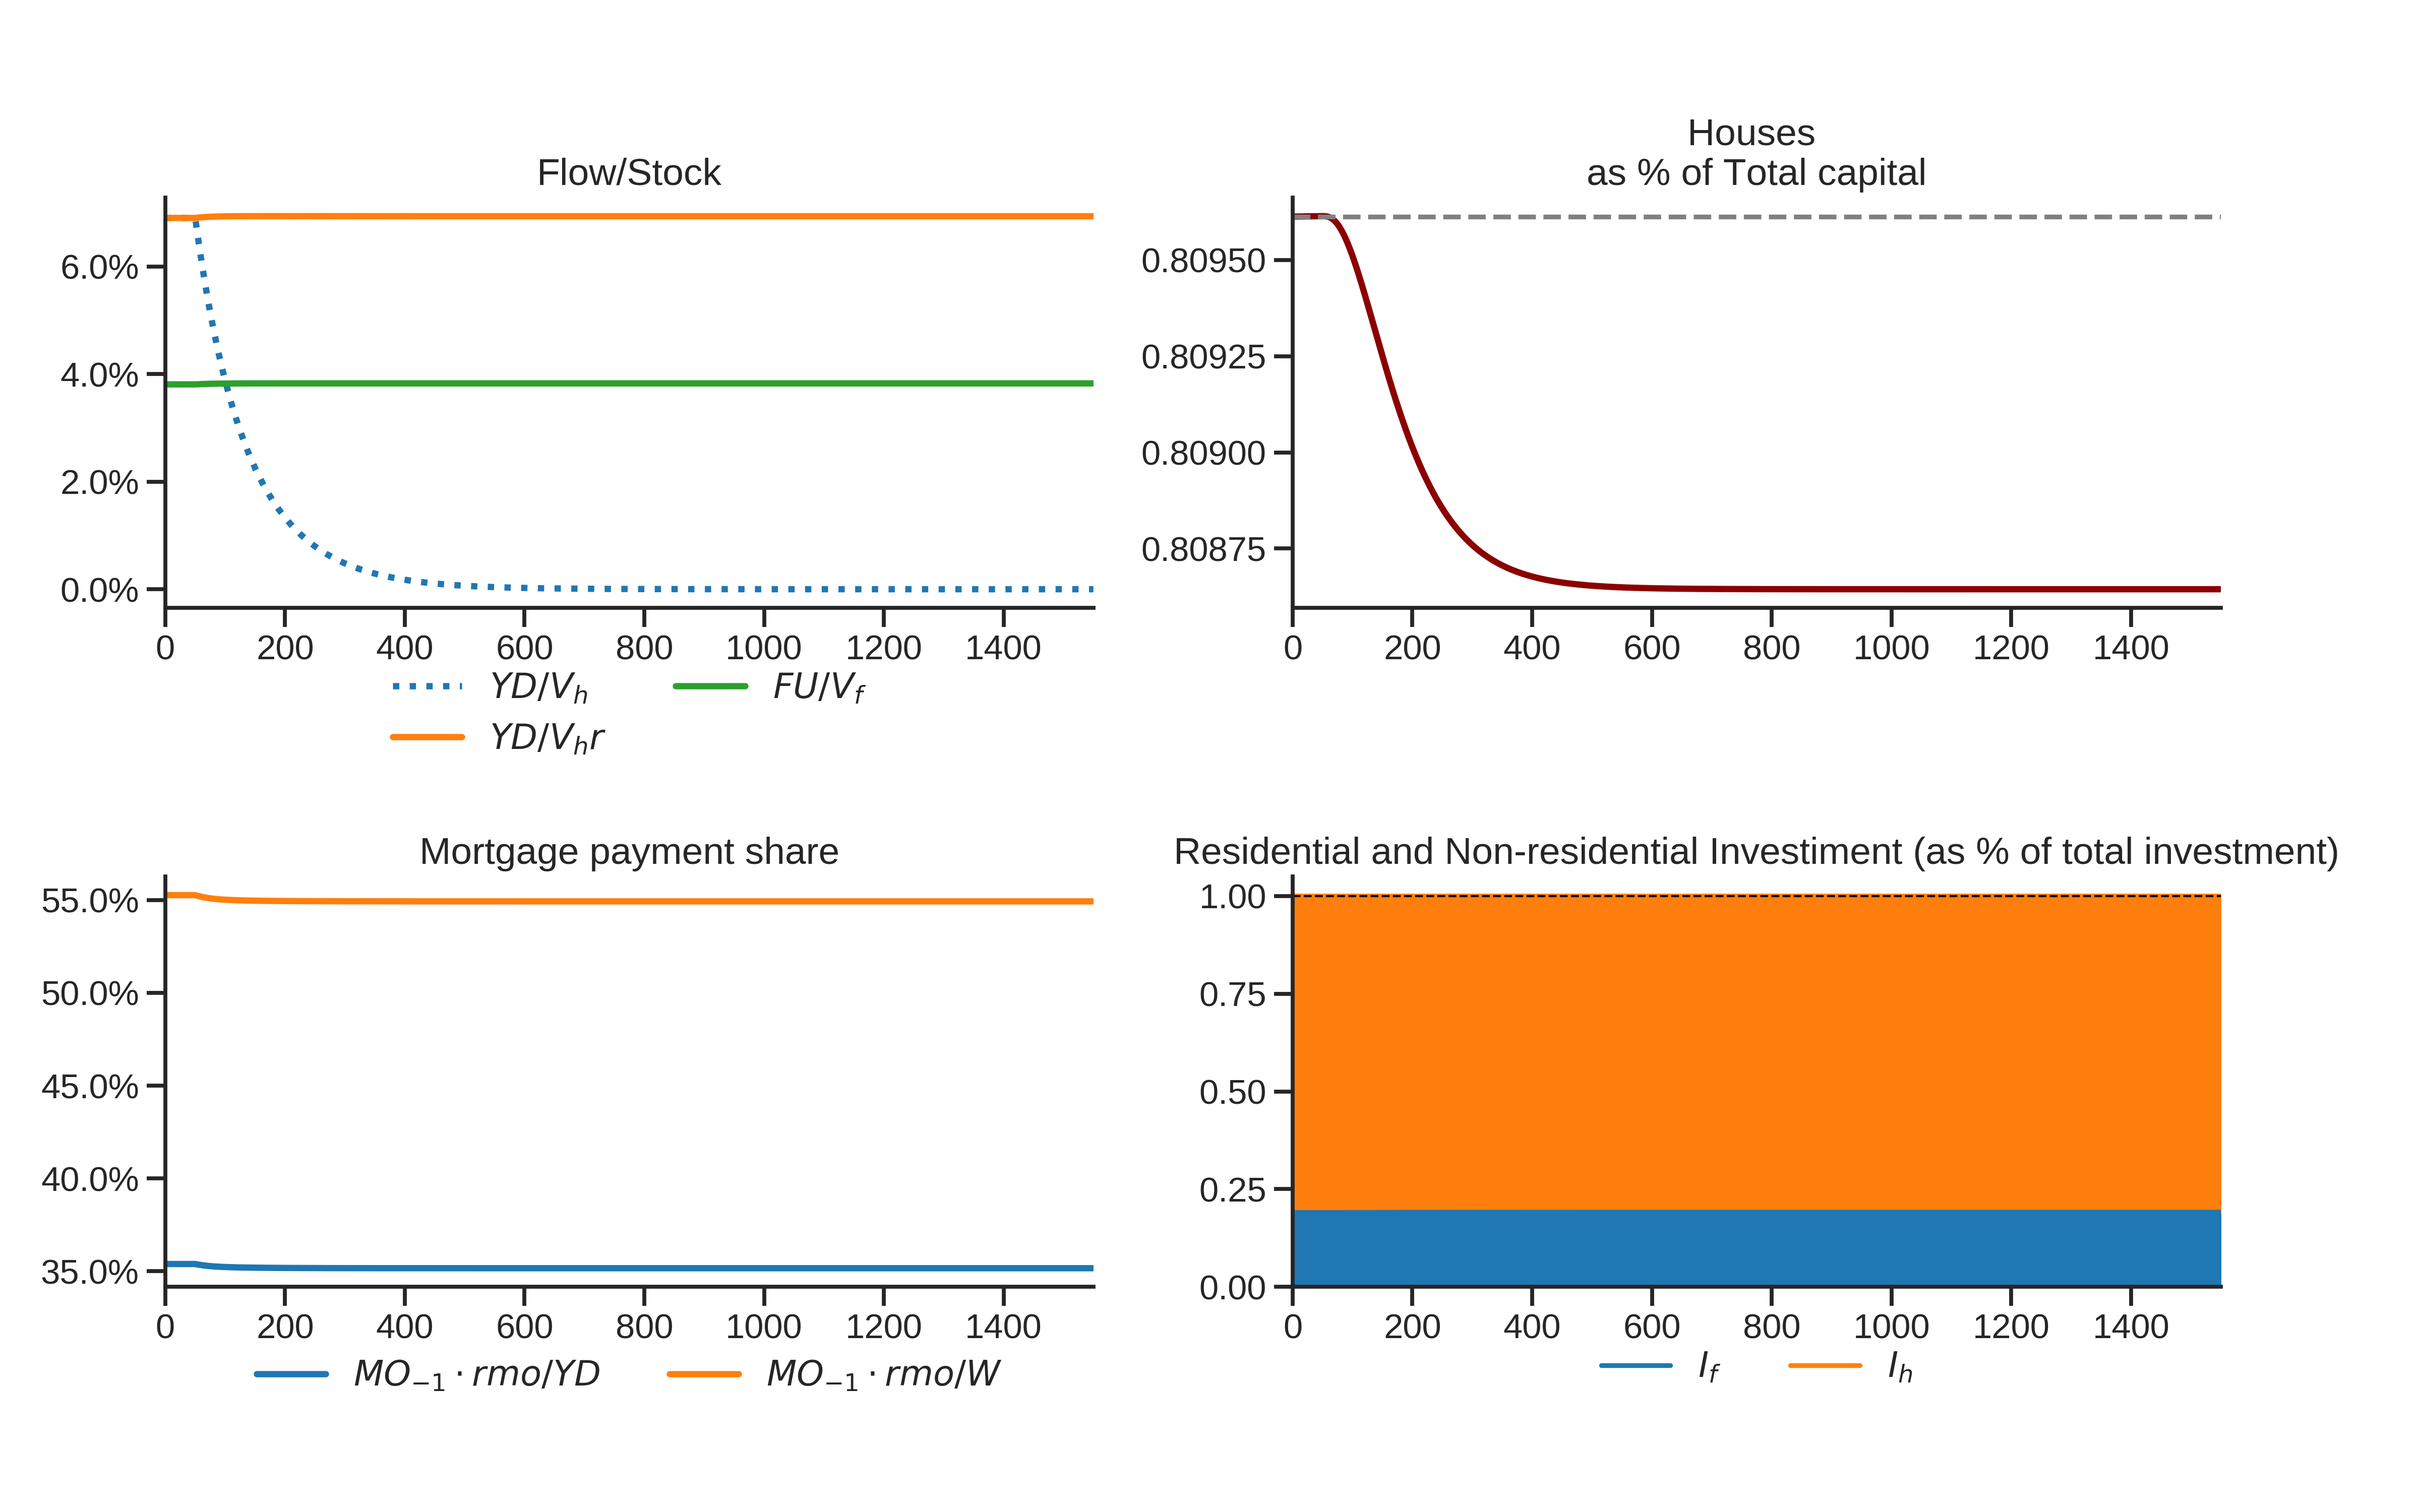
\includegraphics[width=\textwidth]{../../Modelo/Versoes/Shock_4Norms.png}
	\caption*{\textbf{Fonte:} Elaboração própria}
\end{figure}

%Tais resultados, no entanto, são os esperados seguindo a literatura do supermultiplicador sraffiano. A especificidade deste modelo, como destacado, é a existência de dois tipos de estoques de capital uma vez que as famílias também investem. Como resultado do aumento de $g_Z$, há um efeito positivo sobre a taxa de acumulação de modo que a participação do estoque de capital criador de capacidade aumente em relação ao estoque de capital total da economia ($\uparrow k$). 


Tais resultados estão de acordo com \textcite{freitas_growth_2015} e explicitados nas figura \ref{choque_1} e \ref{choque_4} a seguir. A especificidade do presente modelo, como destacado, é a existência de dois tipos de estoques de capital uma vez que as famílias também investem. Um resultado que pode parecer contraintuitivo é que uma maior taxa de crescimento do investimento residencial tem como resultado uma redução  da sua participação \textit{real} no estoque de capital total (isto é, um amento de $K_k$). 
%Adicionalmente, verifica-se um aumento  na participação nominal dos imóveis na presenção de inflação.

\subsection*{Aumento da participação dos salários na renda}
%esse parágrafo ficou bem confuso
%O aumento no \textit{wage-share} gera efeitos positivos sobre a taxa de crescimento da economia e também sobre o grau de utilização, conforme mostra a figura 6(a). No entanto, tais efeitos são temporários uma vez que a taxa de crescimento dos gastos autônomos não é alterada. Isso é refletido no aumento do grau de utilização mesmo estando abaixo do desejado em alguns períodos dada a convergência da taxa de crescimento da economia a $g_Z$ de modo que: (i) taxa de crescimento média é maior que a inicial, mas converge para $g_Z$ no longo prazo; (ii) o aumento na propensão marginal a investir é temporário e retorna ao valor do \textit{baseline}; (iii) grau de utilização converge ao normal mais rapidamente em relação ao choque anterior. 

O aumento no \textit{wage-share} gera efeitos positivos sobre a taxa de crescimento da economia e também sobre o grau de utilização, conforme mostra a figura \ref{choque_2}. No entanto, tais efeitos são temporários uma vez que a taxa de crescimento dos gastos autônomos não é alterada.Com isso temos que: (i) o aumento na propensão marginal a investir é temporário e retorna ao valor do \textit{baseline}; (ii) grau de utilização converge ao normal mais rapidamente em relação ao choque anterior. 


\begin{figure}[H]
	\centering
	\caption{Efeito de uma redistribuição de renda a favor dos lucros}
	\label{choque_2}
	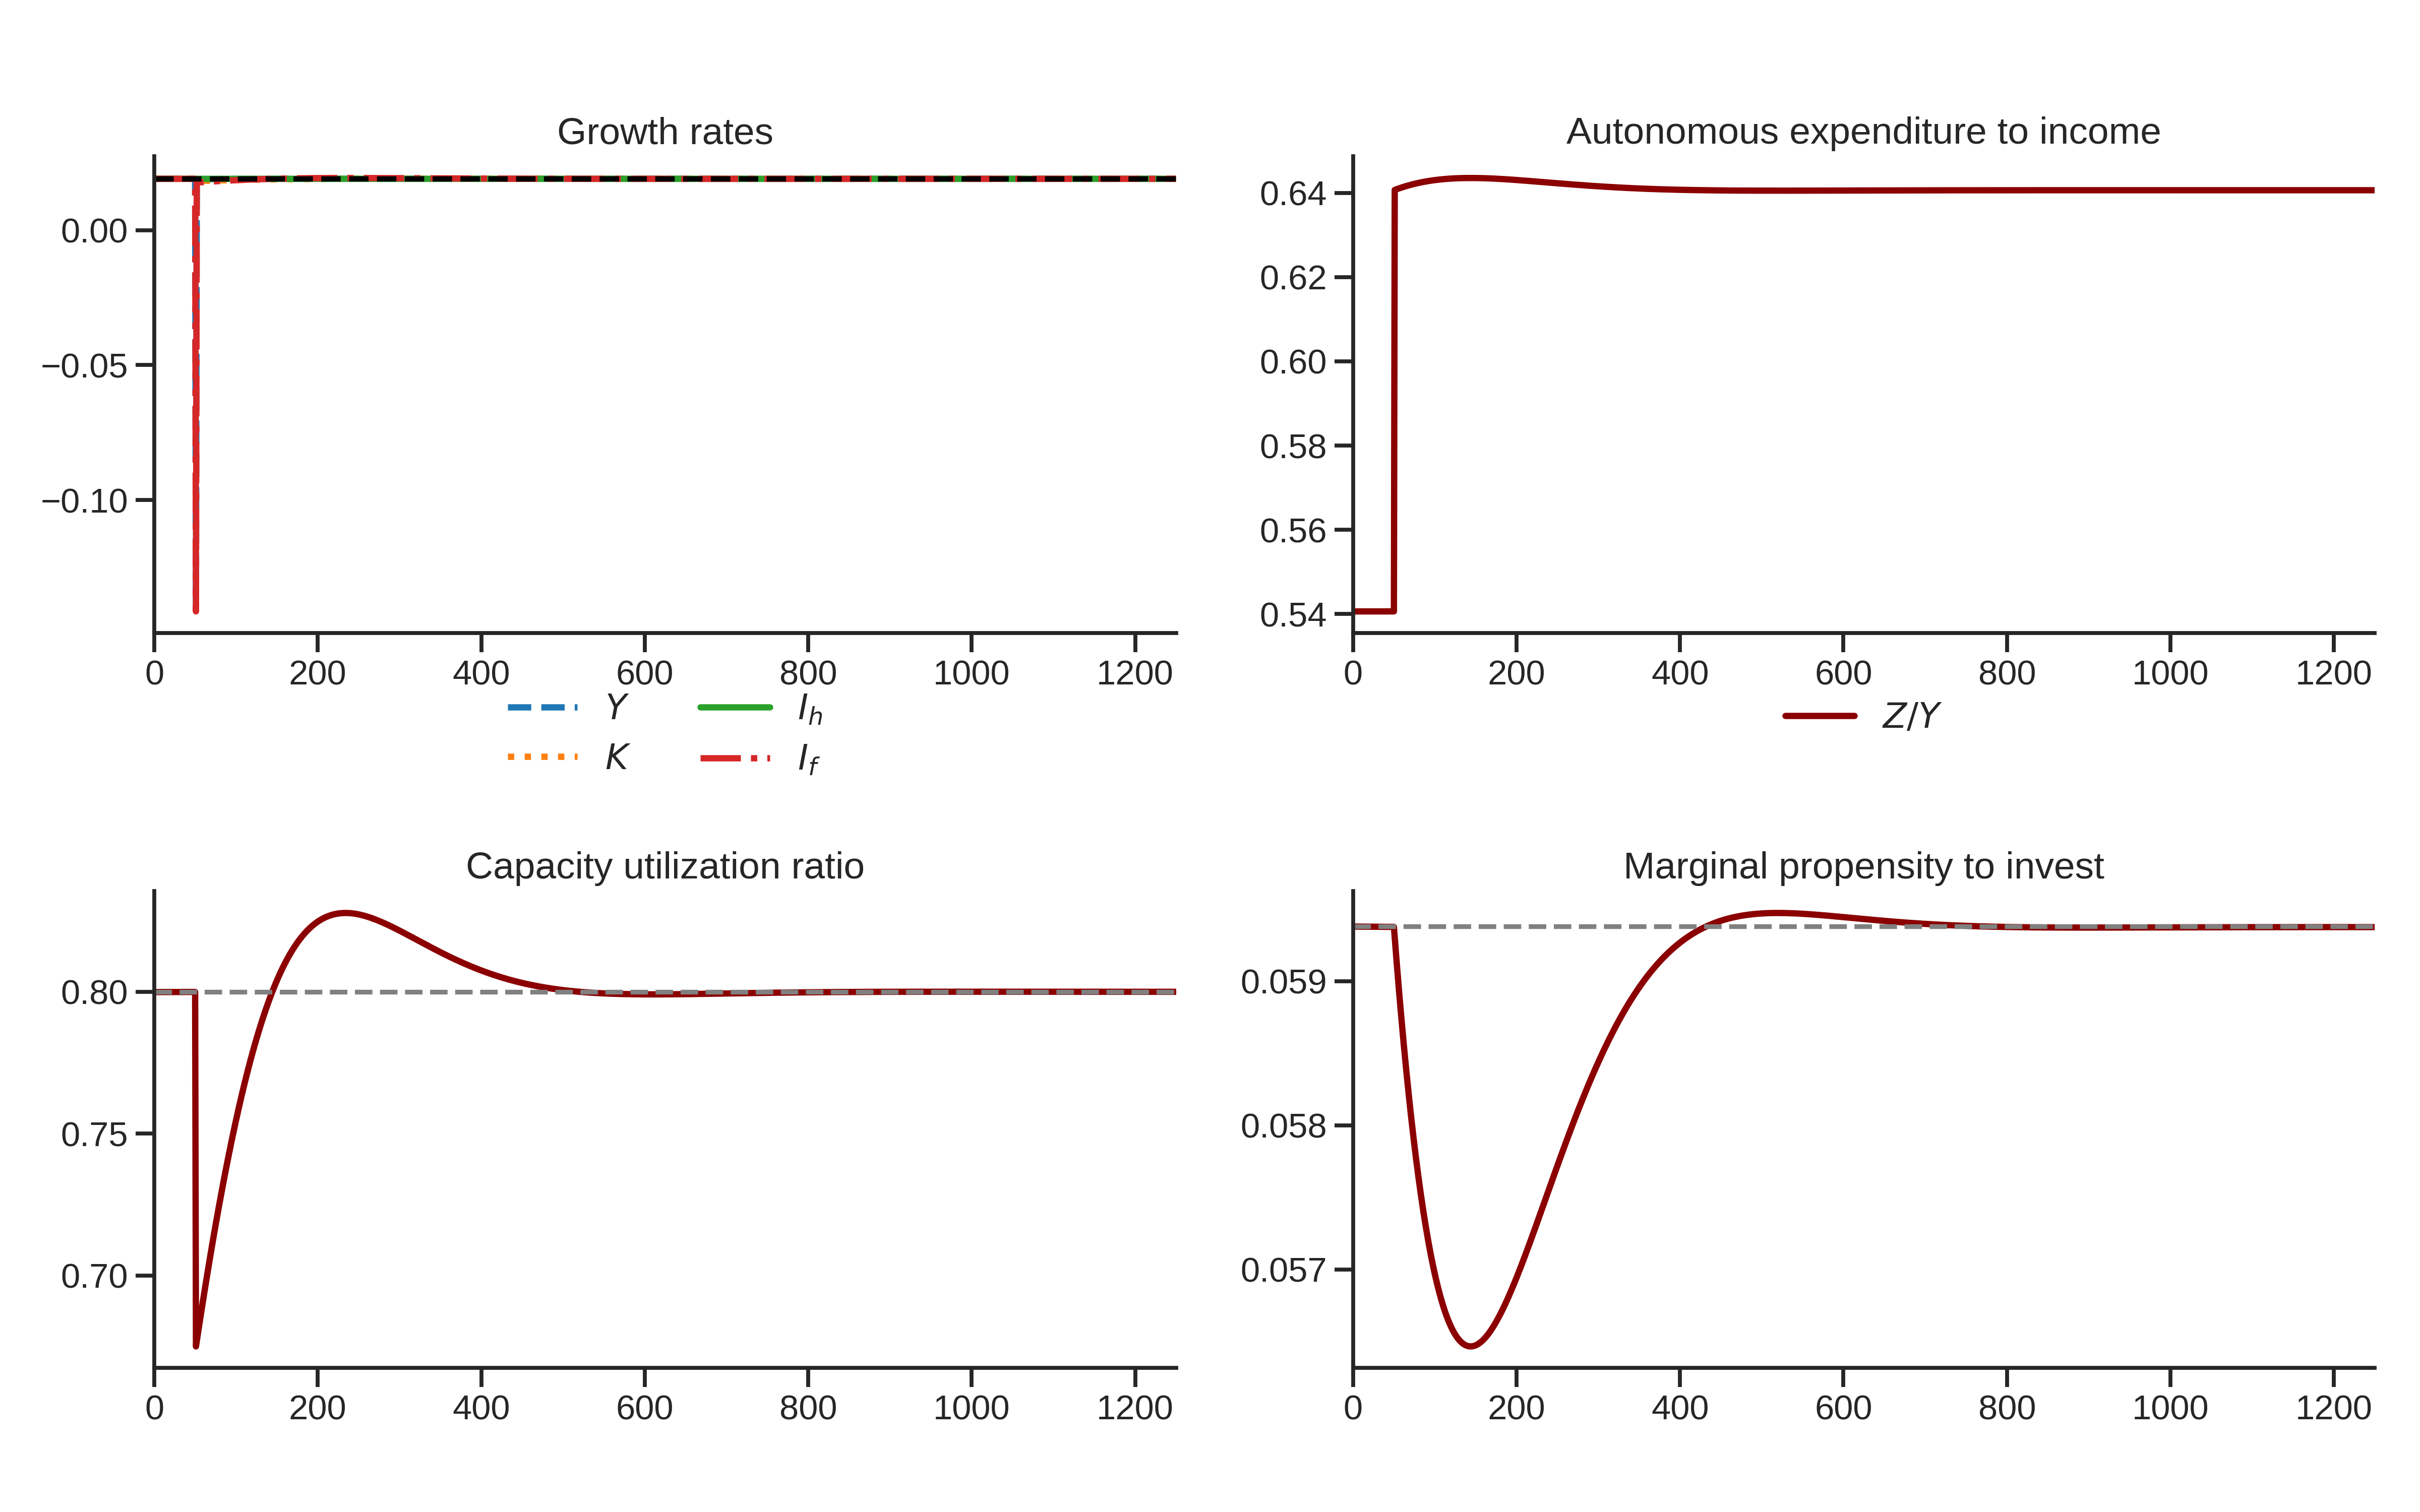
\includegraphics[width=\textwidth]{../../Modelo/Versoes/Shock_2.png}
	\caption*{\textbf{Fonte:} Elaboração própria}
\end{figure}


\begin{figure}[H]
	\centering
	\caption{Efeito de uma redistribuição de renda a favor dos lucros}
	\label{choque_2Norms}
	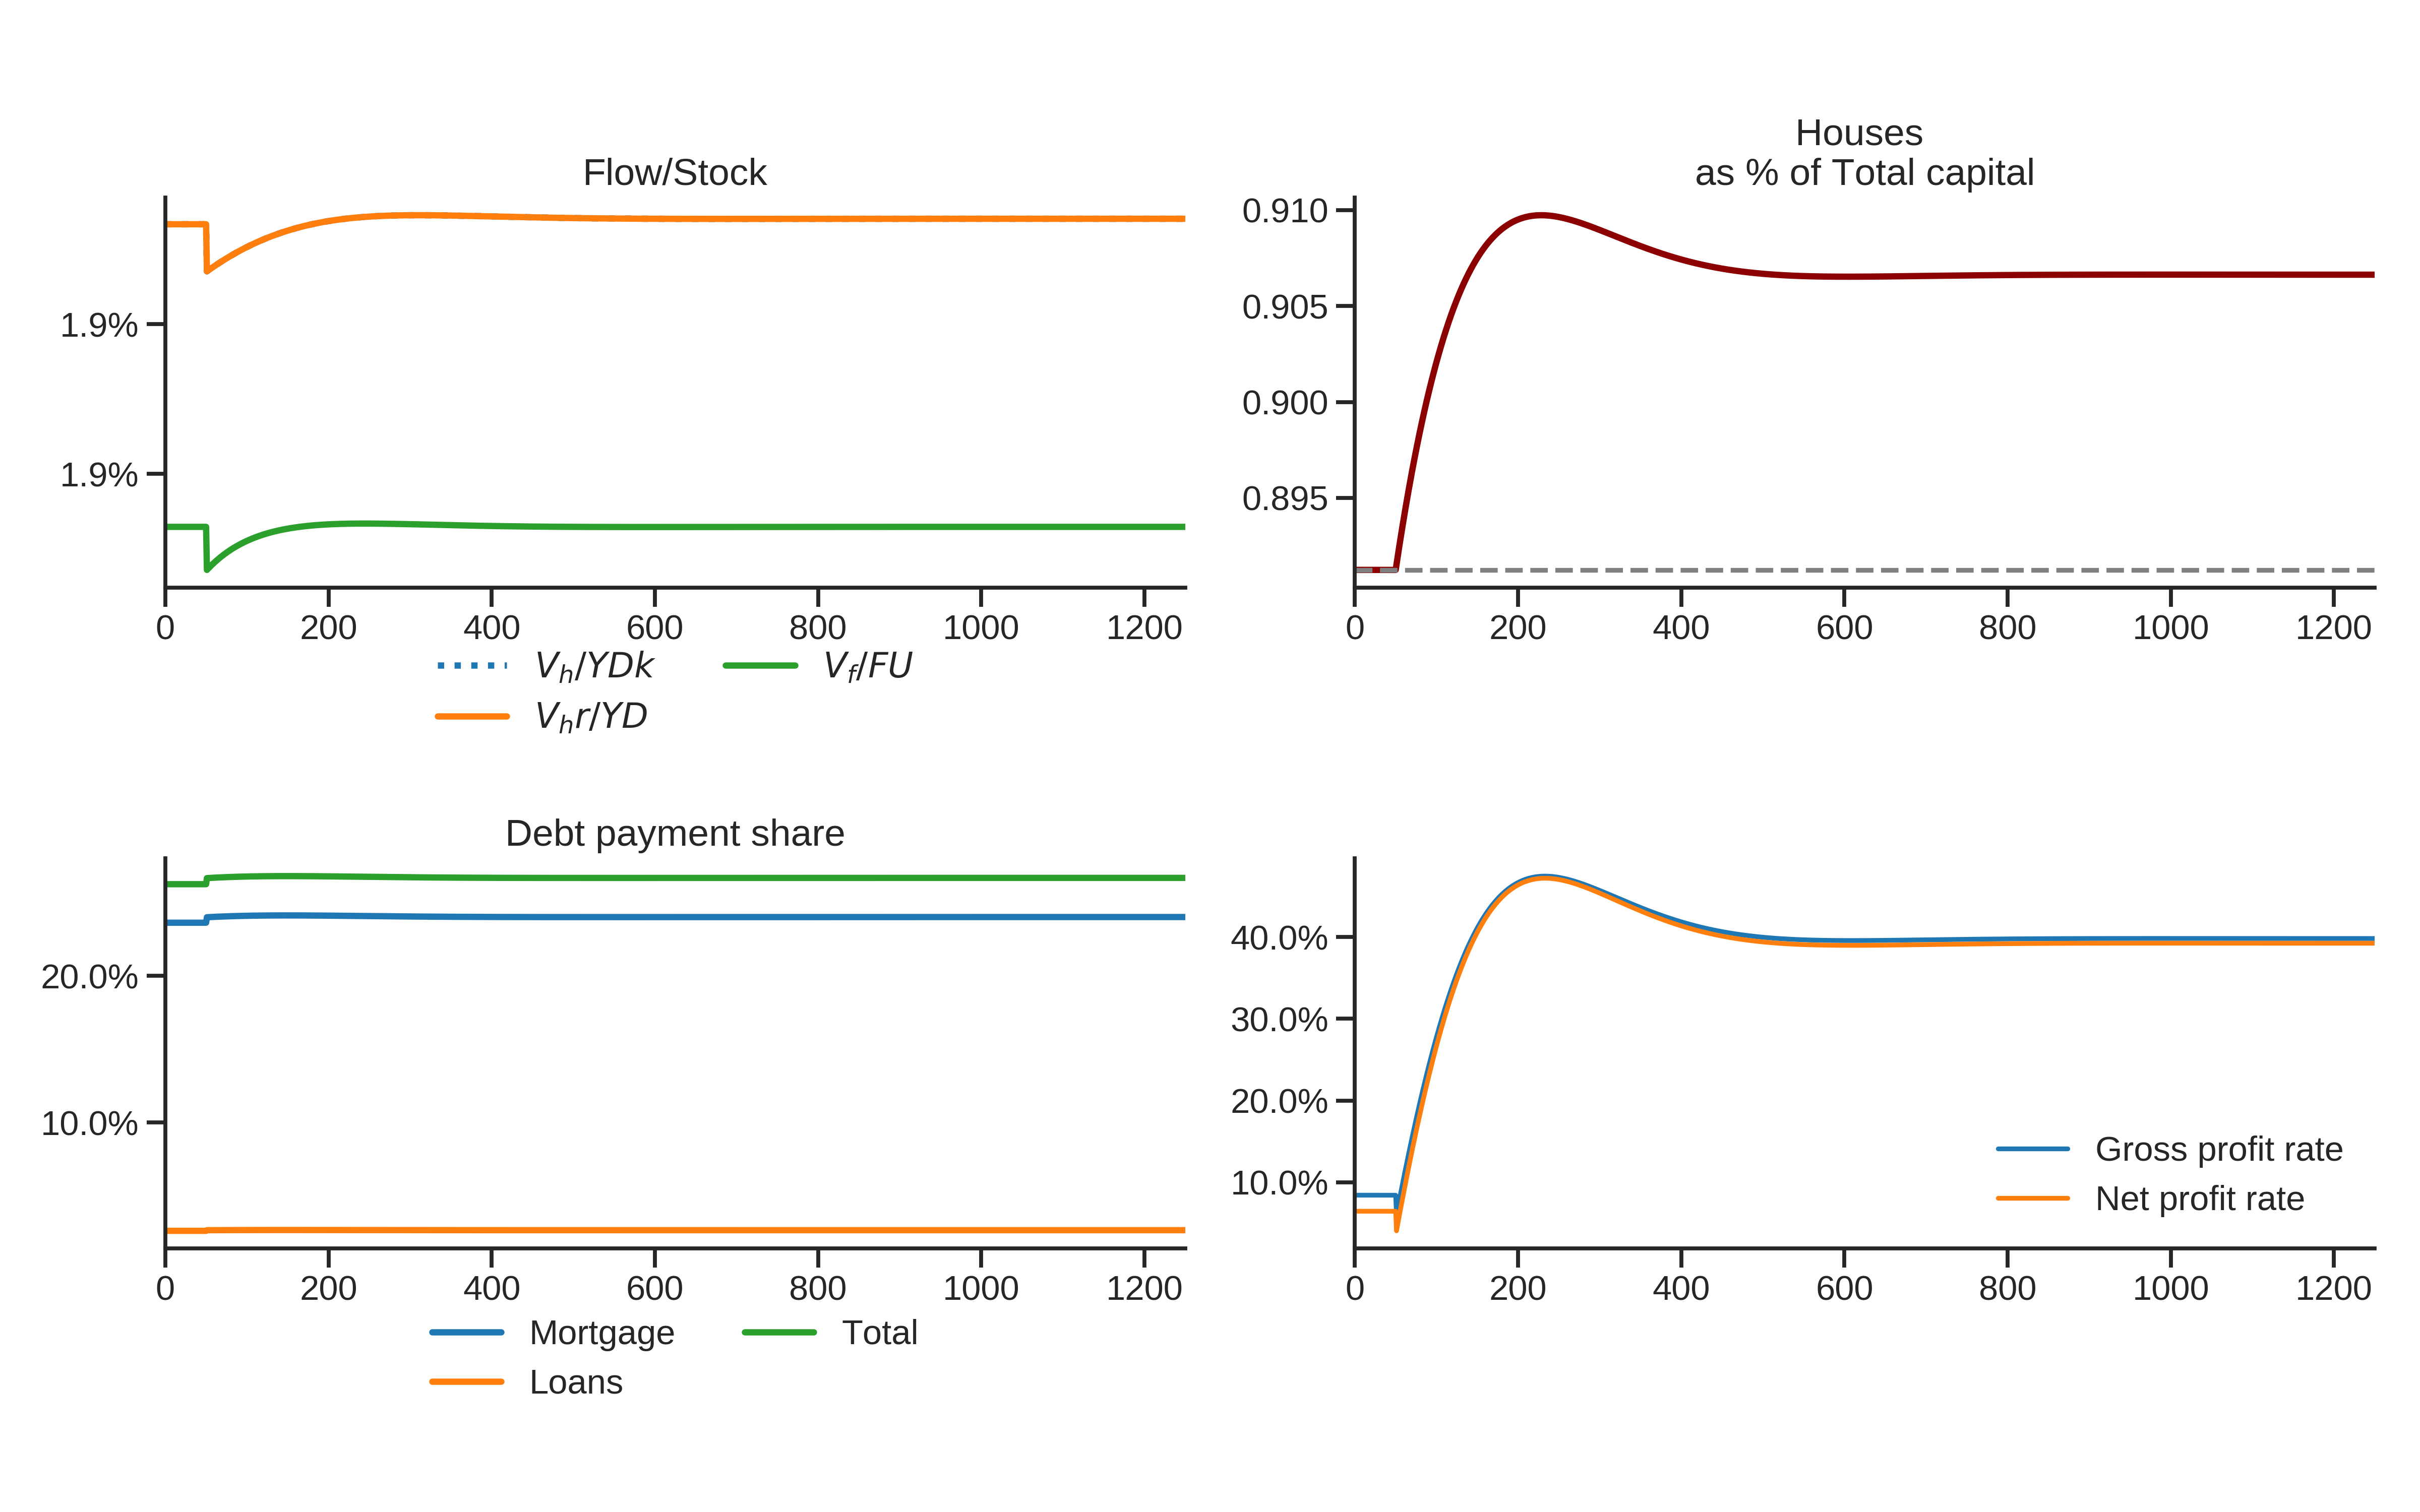
\includegraphics[width=\textwidth]{../../Modelo/Versoes/Shock_2Norms.png}
	\caption*{\textbf{Fonte:} Elaboração própria}
\end{figure}

Por fim, apesar do efeito sobre a taxa de crescimento ser temporário, tem efeitos persistentes sobre a participação do capital das firmas no estoque total de capital da economia. Tal resultado decorre da maior taxa de acumulação no início do choque uma vez que a taxa de crescimento do investimento residencial é mantida constante. 

\subsection*{Aumento da taxa de juros}

Um aumento da taxa de juros hipotecária, ao impactar a taxa própria, não possui efeitos \textbf{persistentes} sobre a taxa de crescimento (figura \ref{choque_3}). Como resultado da menor taxa de crescimento do investimento residencial, a taxa de crescimento do investimento das firmas subreage (\textit{overshooting} negativo) de tal modo que a participação dos imóveis no total do estoque de capital aumenta. Além disso, vale mencionar o maior comprometimento da renda das famílias com pagamento dos juros hipotecários que não é acompanhado de um maior rendimento dos depósitos uma vez que está associado ao aumento do \textit{risk and trouble} e não da taxa básica de juros da economia.

\begin{figure}[H]
	\centering
	\caption{Efeito de Aumento na taxa de juros das hipotecas}
	\label{choque_3}
	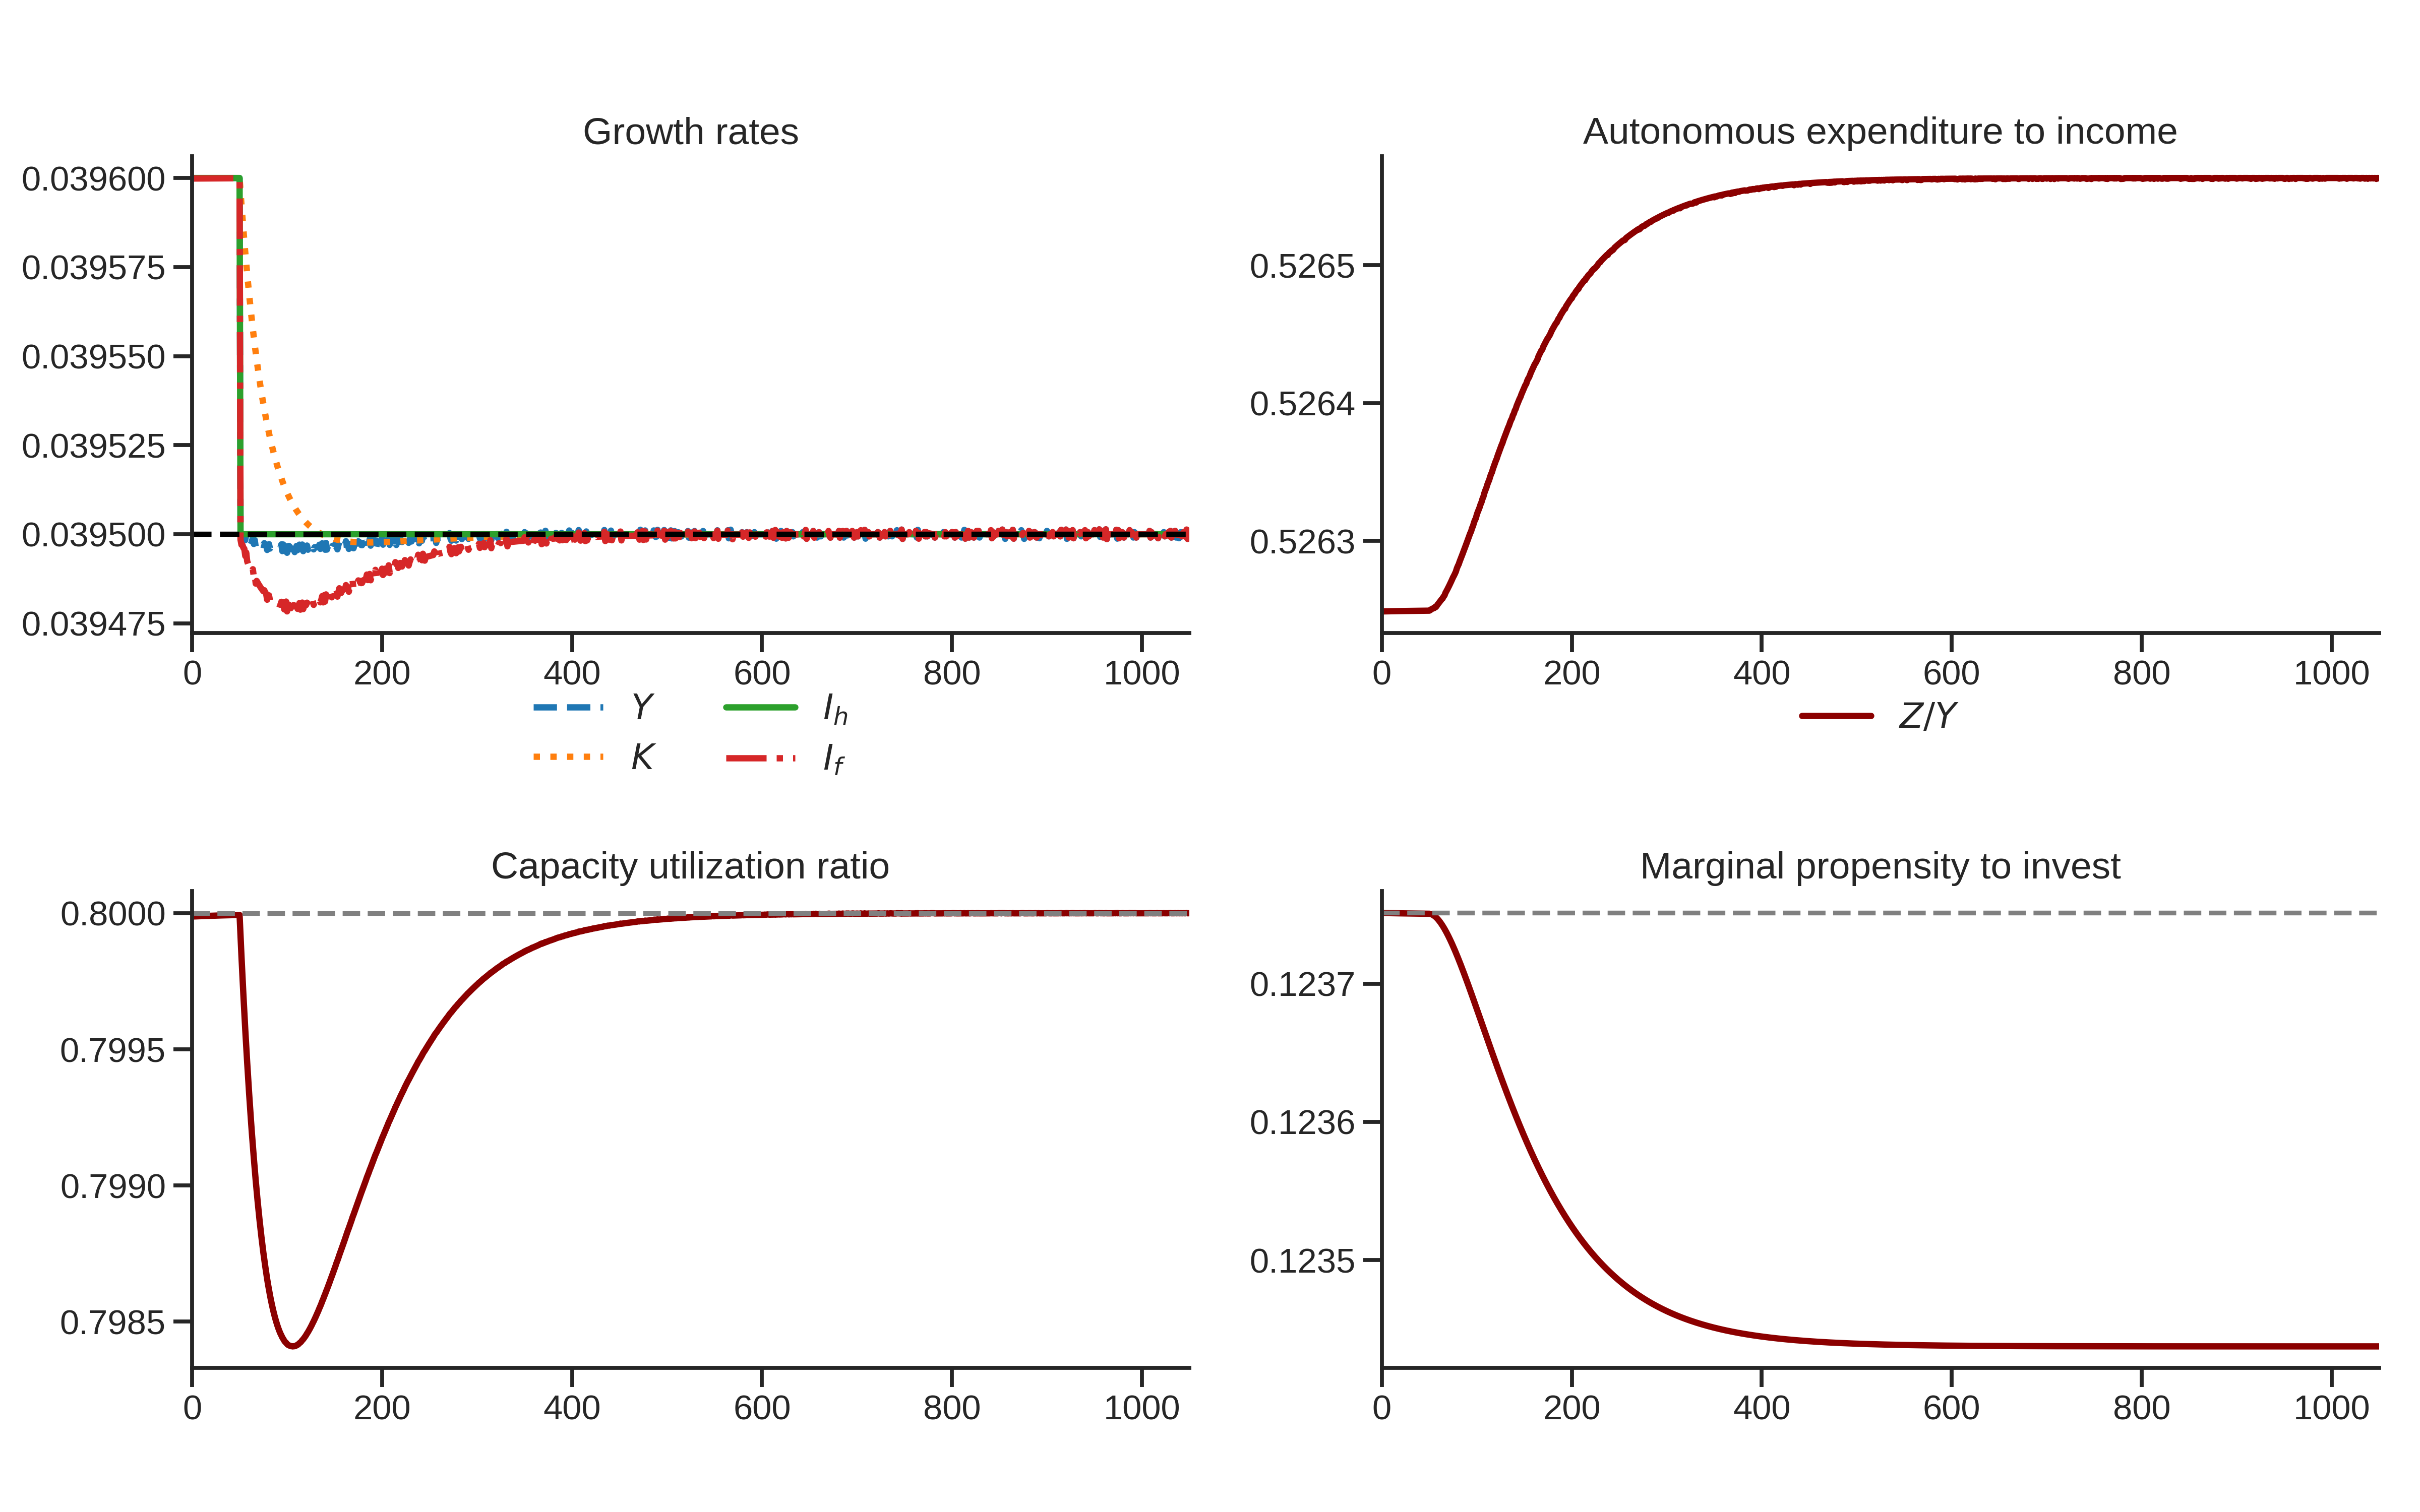
\includegraphics[width=\textwidth]{../../Modelo/Versoes/Shock_3.png}
	\caption*{\textbf{Fonte:} Elaboração própria}
\end{figure}


\begin{figure}[H]
	\centering
	\caption{Efeito de Aumento na taxa de juros das hipotecas}
	\label{choque_3Norms}
	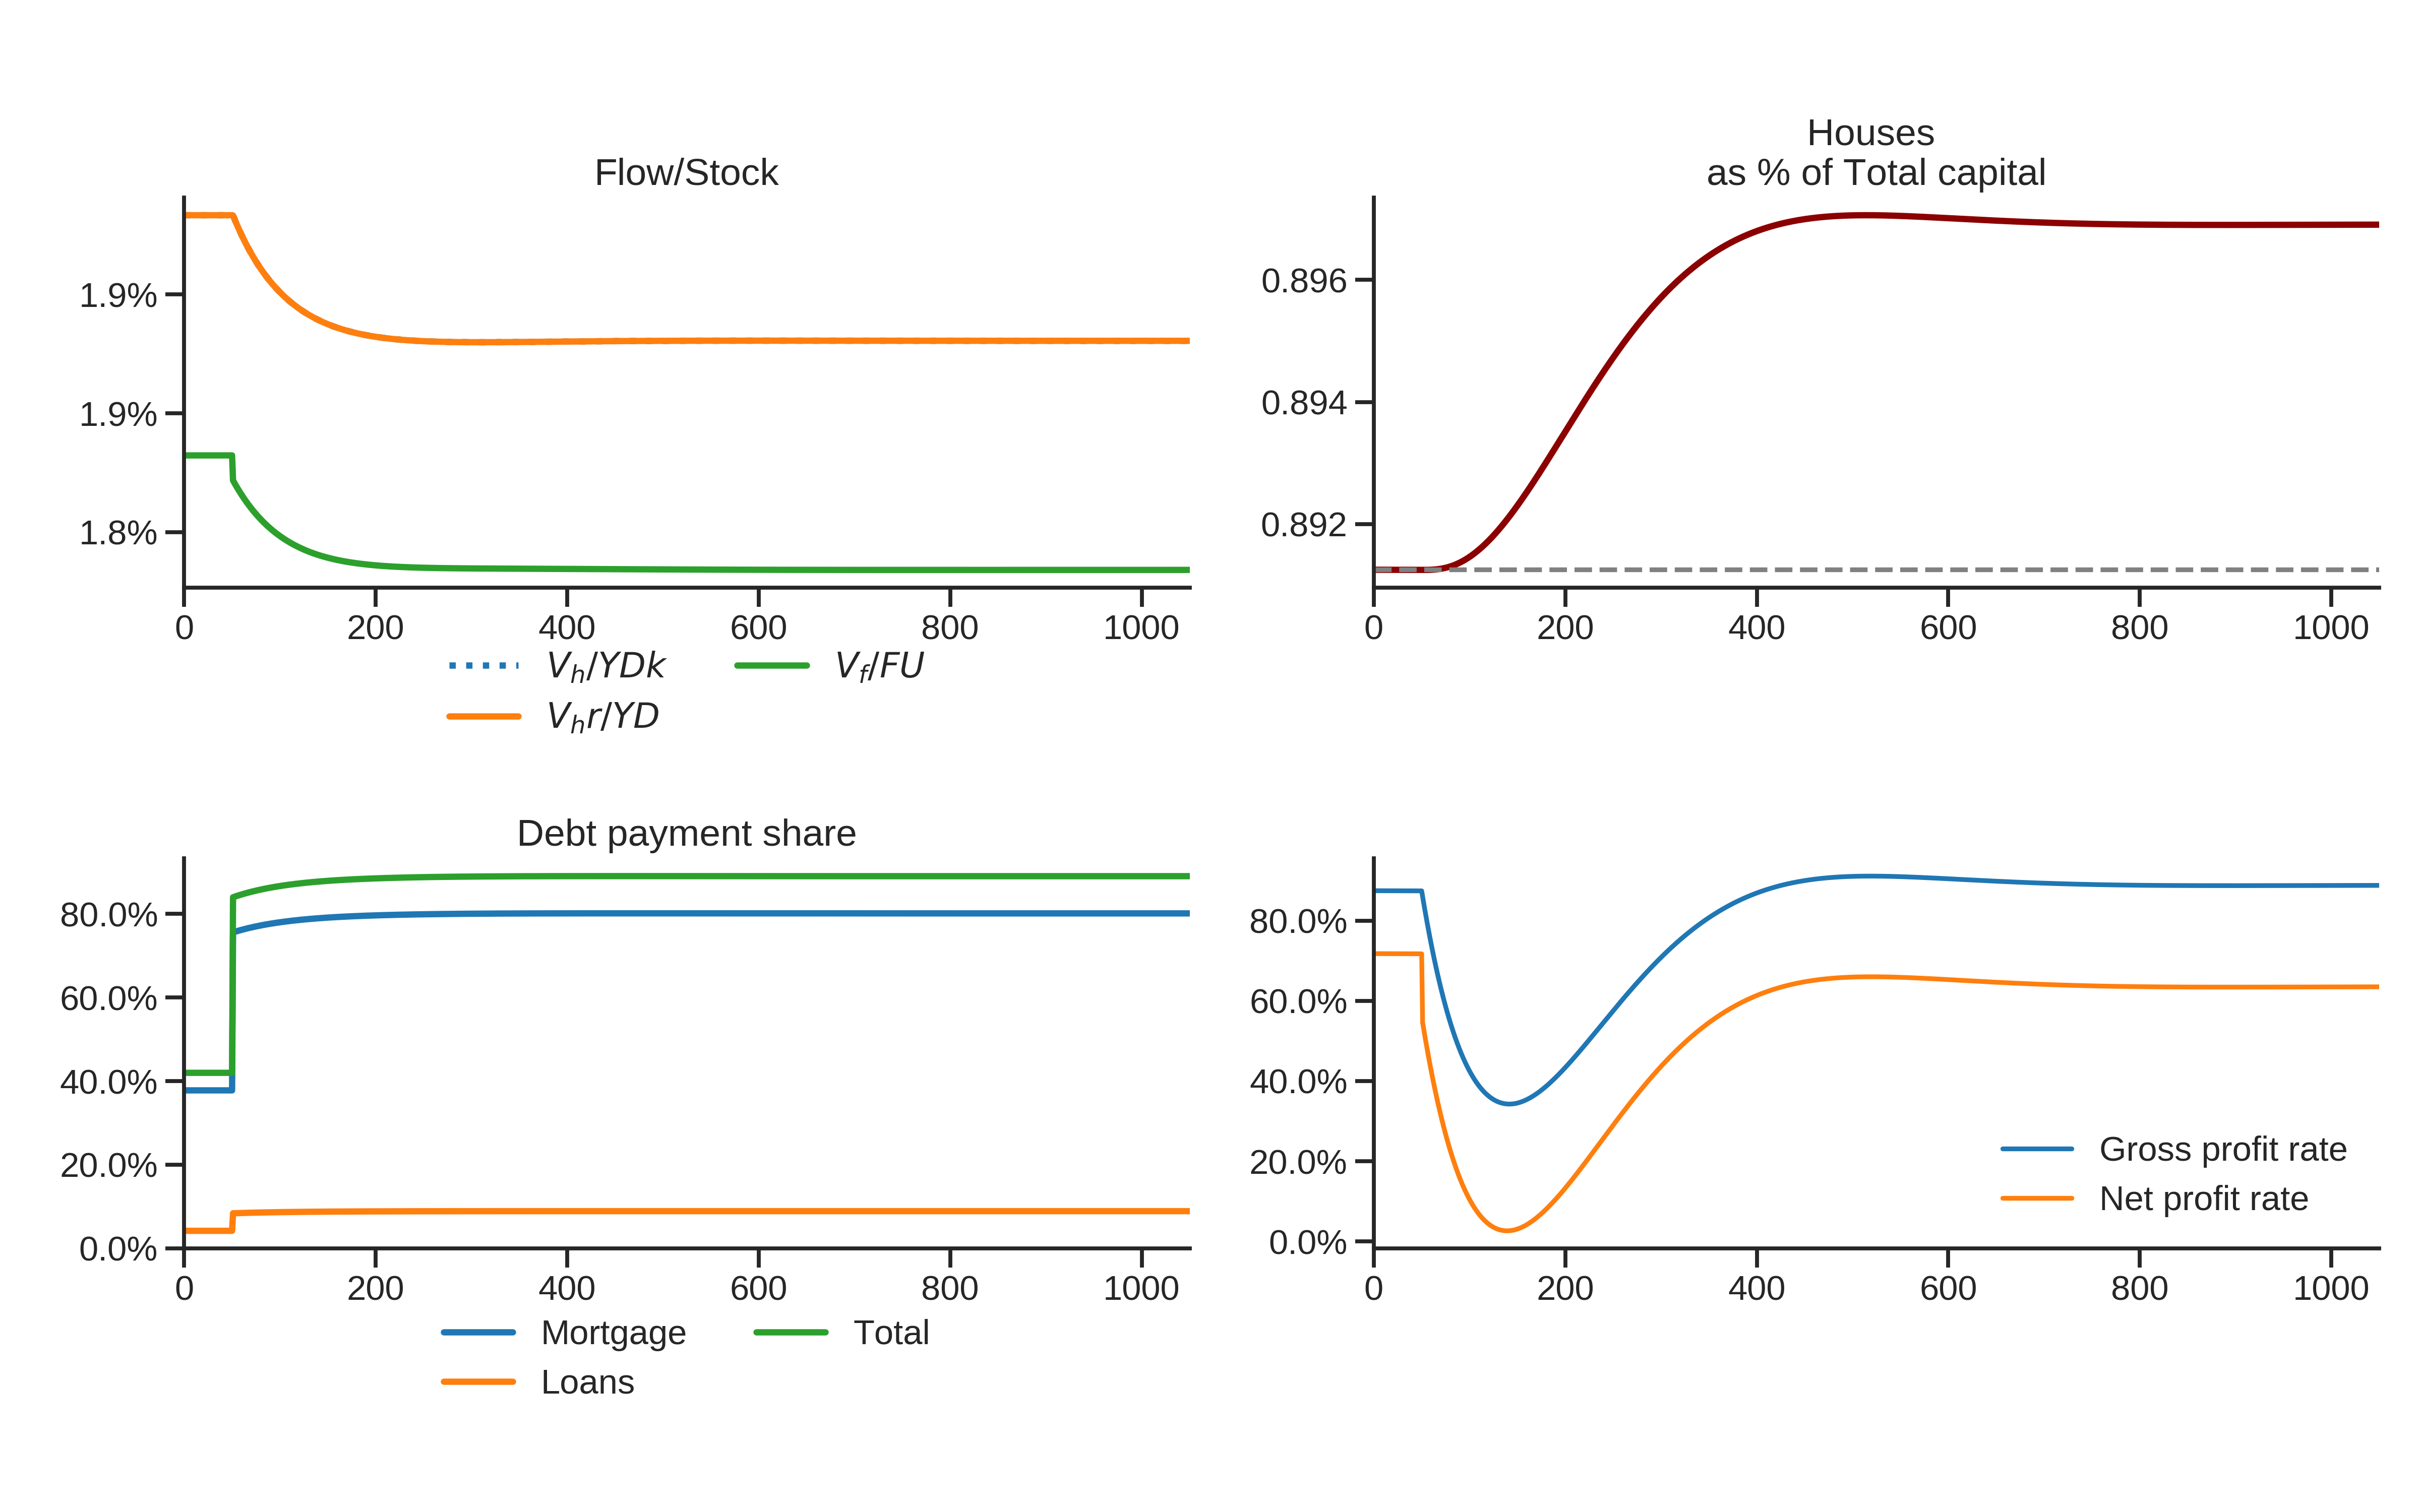
\includegraphics[width=\textwidth]{../../Modelo/Versoes/Shock_3Norms.png}
	\caption*{\textbf{Fonte:} Elaboração própria}
\end{figure}



\begin{table}[H]
    \centering
    \caption{Parâmetros das simulações}
    \label{Resumo_Simulacao}
	\begin{tabular}{c}
\toprule
{} &  Base scenario &  $\Delta \phi_0$ &  $\Delta \omega$ &   $\Delta rm$ &  $\Delta $ Infla \\
\midrule
\textbf{alpha    } &   1,000000e+00 &     1,000000e+00 &     1,000000e+00 &  1,000000e+00 &     1,000000e+00 \\
\textbf{alpha_2  } &   3,000000e-01 &     3,000000e-01 &     3,000000e-01 &  3,000000e-01 &     3,000000e-01 \\
\textbf{gamma_F  } &   9,000000e-01 &     9,000000e-01 &     9,000000e-01 &  9,000000e-01 &     9,000000e-01 \\
\textbf{gamma_u  } &   1,000000e-02 &     1,000000e-02 &     1,000000e-02 &  1,000000e-02 &     1,000000e-02 \\
\textbf{omega    } &   3,000000e-01 &     3,000000e-01 &     2,500000e-01 &  3,000000e-01 &     3,000000e-01 \\
\textbf{rm       } &   2,000000e-02 &     2,000000e-02 &     2,000000e-02 &  2,000000e-02 &     2,000000e-02 \\
\textbf{spread_l } &   0,000000e+00 &     0,000000e+00 &     0,000000e+00 &  0,000000e+00 &     0,000000e+00 \\
\textbf{spread_mo} &   0,000000e+00 &     0,000000e+00 &     0,000000e+00 &  5,000000e-03 &     0,000000e+00 \\
\textbf{un       } &   8,000000e-01 &     8,000000e-01 &     8,000000e-01 &  8,000000e-01 &     8,000000e-01 \\
\textbf{v        } &   2,500000e+00 &     2,500000e+00 &     2,500000e+00 &  2,500000e+00 &     2,500000e+00 \\
\textbf{phi_0    } &   4,000000e-02 &     5,000000e-02 &     4,000000e-02 &  4,000000e-02 &     4,000000e-02 \\
\textbf{phi_1    } &   2,000000e-02 &     2,000000e-02 &     2,000000e-02 &  2,000000e-02 &     2,000000e-02 \\
\textbf{phparam  } &   1,000000e+00 &     1,000000e+00 &     1,000000e+00 &  1,000000e+00 &     1,000000e+00 \\
\textbf{infla    } &   0,000000e+00 &     0,000000e+00 &     0,000000e+00 &  0,000000e+00 &     1,000000e-02 \\
\textbf{gZn      } &   3,900000e-02 &     3,922000e-02 &     3,900000e-02 &  3,900000e-02 &     3,900000e-02 \\
\textbf{_K_f__1  } &   4,244058e+19 &     1,082934e+44 &     3,585057e+30 &  1,974191e+37 &     7,896508e+45 \\
\textbf{_M__1    } &  -1,326991e+20 &    -1,611049e+44 &    -1,223085e+31 & -6,225215e+37 &    -2,427467e+46 \\
\textbf{_MO__1   } &   1,855990e+20 &     3,598007e+44 &     1,704715e+31 &  8,659263e+37 &     3,432732e+46 \\
\textbf{_Lf__1   } &  -3,182981e+20 &    -5,209056e+44 &    -2,927800e+31 & -1,488448e+38 &    -5,860199e+46 \\
\textbf{_h__1    } &   1,240000e-01 &     1,550000e-01 &     1,240000e-01 &  1,230000e-01 &     1,240000e-01 \\
\textbf{_L__1    } &  -3,182981e+20 &    -5,209056e+44 &    -2,927800e+31 & -1,488448e+38 &    -5,860199e+46 \\
\textbf{_K_HD__1 } &   1,855990e+20 &     3,598007e+44 &     1,704715e+31 &  8,659263e+37 &     3,432732e+46 \\
\textbf{_I_h__1  } &   7,069758e+18 &     1,700278e+43 &     6,493526e+29 &  3,290437e+36 &     1,313996e+45 \\
\textbf{_ph__1   } &   1,000000e+00 &     1,000000e+00 &     1,000000e+00 &  1,000000e+00 &     3,004272e+06 \\
\bottomrule
\end{tabular}

    \caption*{\textbf{Fonte:} Elaboração própria}
\end{table}

